\section{Applications}

From the realistic rivers and oceans in the open world games to small water mechanism in puzzle games,
water is a common element of the background settings in many video games.
However, the types of object that could interact with water or the ways that they can do so in games are usually very limited.
Apart from the designs of the game, one big factor limiting the freedom of the interaction with water is on the technical side \cite{kellomaki2012water}.
Due to technical limitations, game developers lack the ways to fully simulate the water interactions and have to often manually overwrite the physical behaviors, which inevitably causes critical glitches \cite{RedditAssassin}.
With our method, game developers could arbitrarily put objects into water bodies without having to worry about physical glitches.

Figure \ref{boat-sample} shows an example of such application.
Without having to write any additional codes, just by keeping loading heavy balls onto the boat, the sunk depth of the boat automatically increases.
This can be seen clearly from the intersection of the water surface and the boat's interior surface.

\begin{figure}[htb]
	\centering
	\begin{subcaptionblock}{0.46\textwidth}
		\centering
		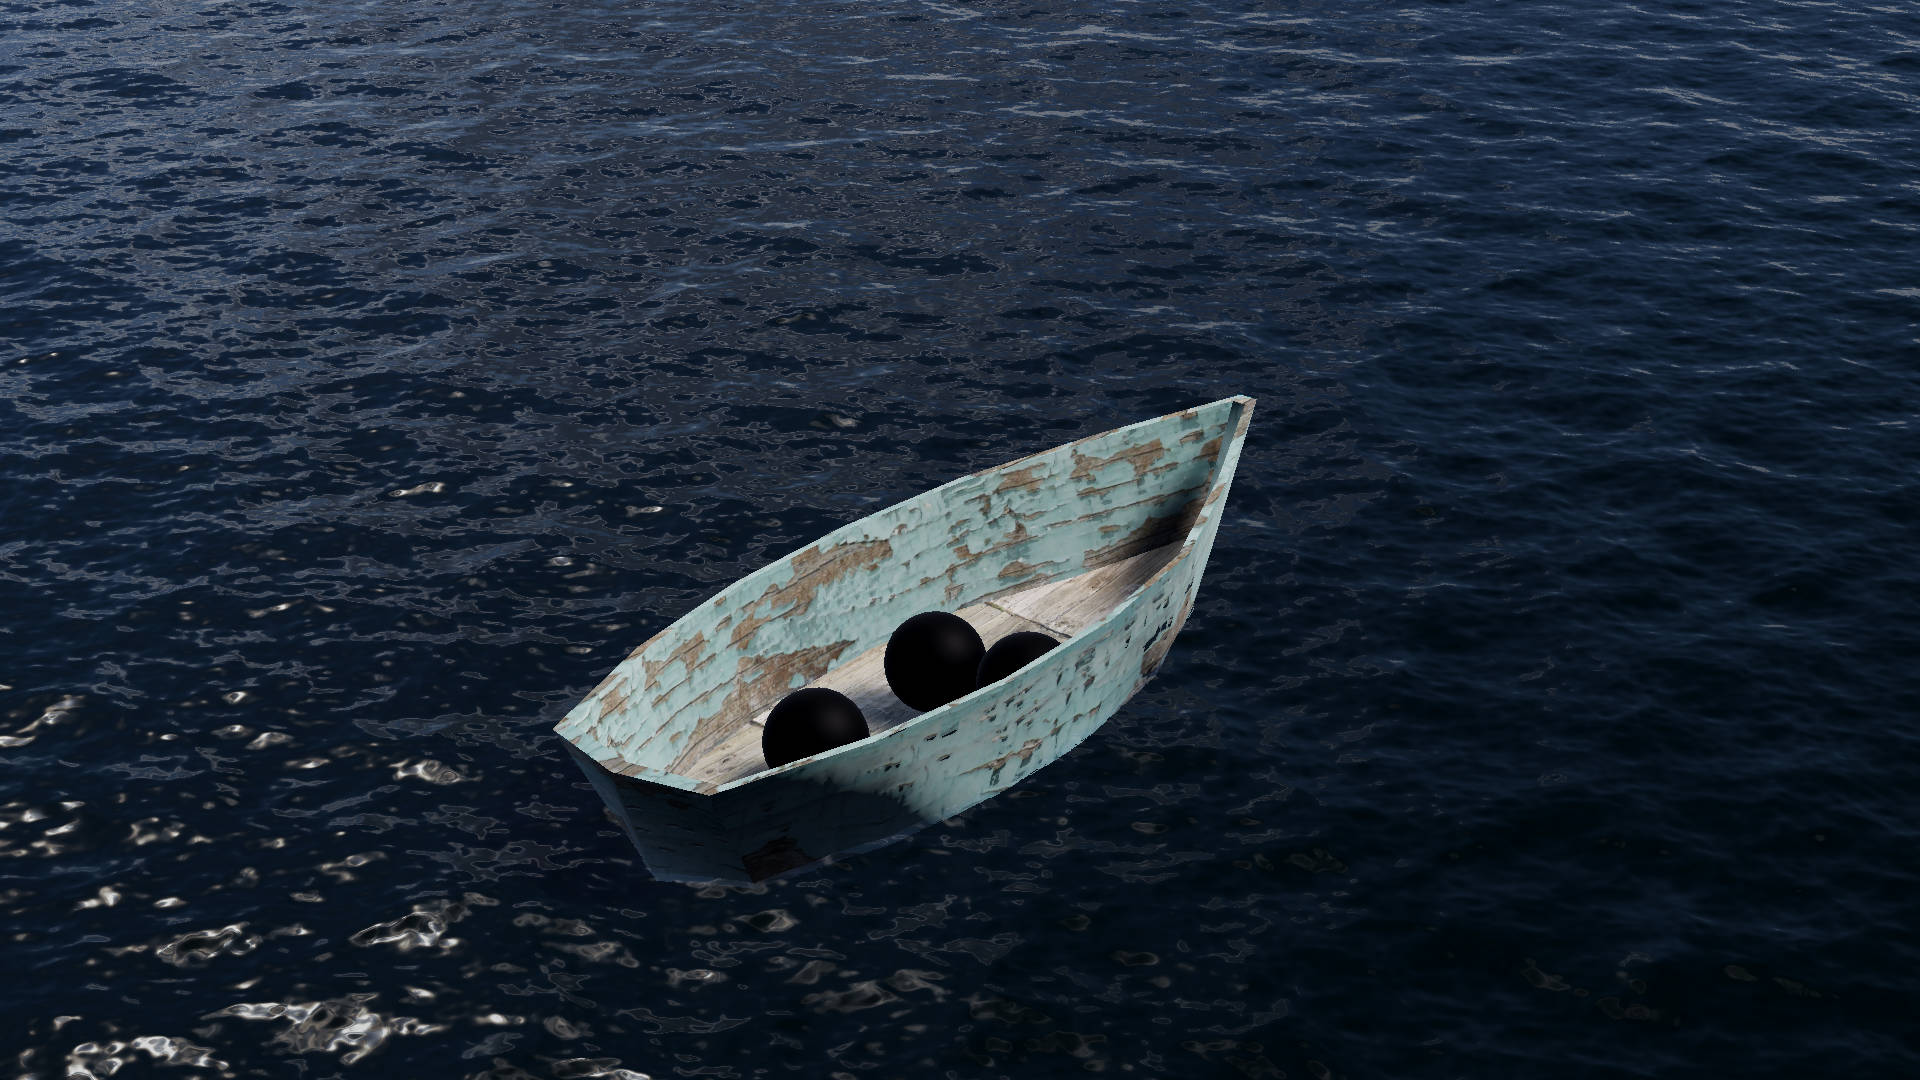
\includegraphics[height=1in]{figures/light-boat.jpg}
		\caption{A boat containing a few balls.}
	\end{subcaptionblock}
	\begin{subcaptionblock}{0.46\textwidth}
		\centering
		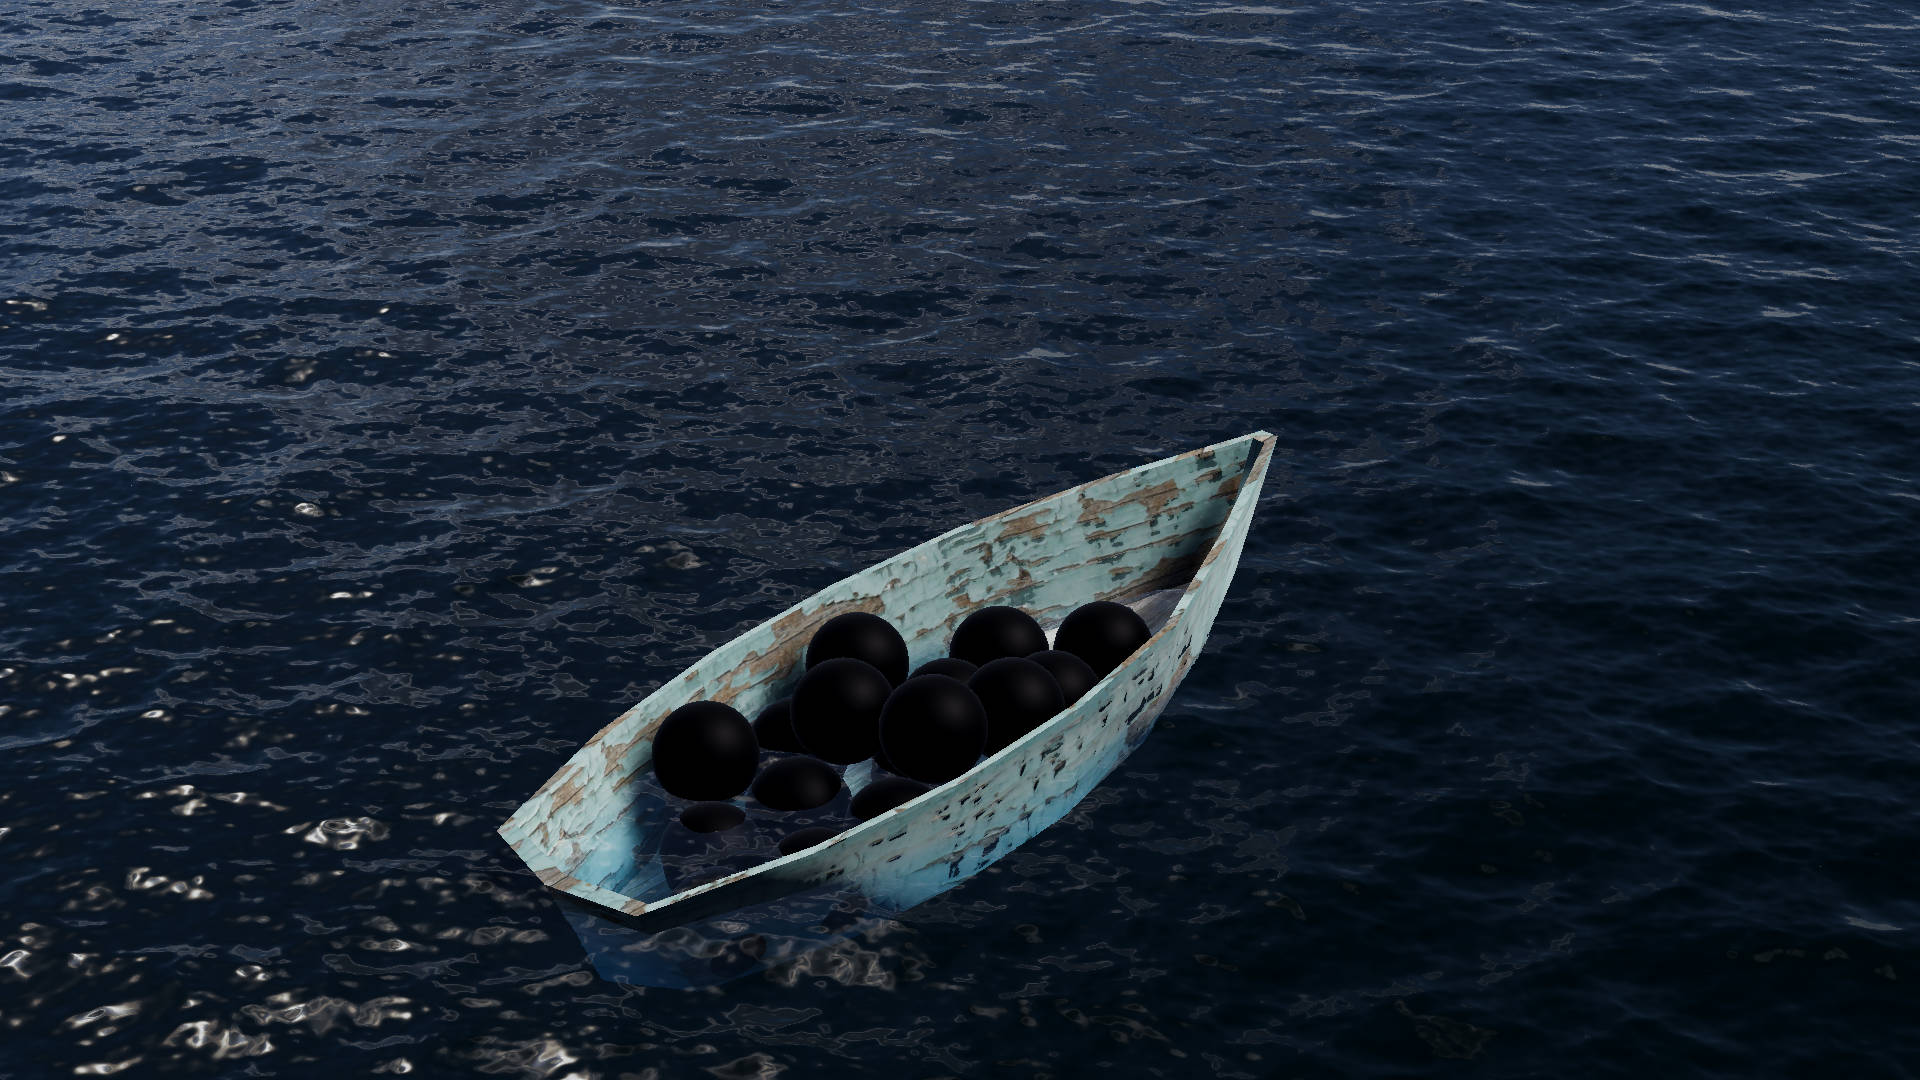
\includegraphics[height=1in]{figures/heavy-boat.jpg}
		\caption{The same boat containing many balls.}
	\end{subcaptionblock}
	\caption{Loading more balls onto the boat increases its depth.}
	\label{boat-sample}
\end{figure}

When applied in real game design, this extra freedom could allow game designers to create more complex mechanisms.
It is clear that often an open mechanism tends to lead to emergent behaviors \cite{sweetser2006emergent}, thus increasing the fun of the game.